%% This is a skeleton file demonstrating the use of IEEEtran.cls to generate 
%% the final manuscript for "VI Iberian Meeting on Computational Electromagnetics".
%% (requires IEEEtran.cls version 1.7 or later) with an IEEE journal paper.
%%

% Some very useful LaTeX packages include:
% (uncomment the ones you want to load)

% *** MISC UTILITY PACKAGES ***
%
%\usepackage{ifpdf}
% Heiko Oberdiek's ifpdf.sty is very useful if you need conditional
% compilation based on whether the output is pdf or dvi.
% usage:
% \ifpdf
%   % pdf code
% \else
%   % dvi code
% \fi
% The latest version of ifpdf.sty can be obtained from:
% http://www.ctan.org/tex-archive/macros/latex/contrib/oberdiek/
% Also, note that IEEEtran.cls V1.7 and later provides a builtin
% \ifCLASSINFOpdf conditional that works the same way.
% When switching from latex to pdflatex and vice-versa, the compiler may
% have to be run twice to clear warning/error messages.


% *** CITATION PACKAGES ***
%
%\usepackage{cite}
% cite.sty was written by Donald Arseneau
% V1.6 and later of IEEEtran pre-defines the format of the cite.sty package
% \cite{} output to follow that of IEEE. Loading the cite package will
% result in citation numbers being automatically sorted and properly
% "compressed/ranged". e.g., [1], [9], [2], [7], [5], [6] without using
% cite.sty will become [1], [2], [5]--[7], [9] using cite.sty. cite.sty's
% \cite will automatically add leading space, if needed. Use cite.sty's
% noadjust option (cite.sty V3.8 and later) if you want to turn this off.
% cite.sty is already installed on most LaTeX systems. Be sure and use
% version 4.0 (2003-05-27) and later if using hyperref.sty. cite.sty does
% not currently provide for hyperlinked citations.
% The latest version can be obtained at:
% http://www.ctan.org/tex-archive/macros/latex/contrib/cite/
% The documentation is contained in the cite.sty file itself.


% *** MATH PACKAGES ***
%
%\usepackage[cmex10]{amsmath}
% A popular package from the American Mathematical Society that provides
% many useful and powerful commands for dealing with mathematics. If using
% it, be sure to load this package with the cmex10 option to ensure that
% only type 1 fonts will utilized at all point sizes. Without this option,
% it is possible that some math symbols, particularly those within
% footnotes, will be rendered in bitmap form which will result in a
% document that can not be IEEE Xplore compliant!
%
% Also, note that the amsmath package sets \interdisplaylinepenalty to 10000
% thus preventing page breaks from occurring within multiline equations. Use:
%\interdisplaylinepenalty=2500
% after loading amsmath to restore such page breaks as IEEEtran.cls normally
% does. amsmath.sty is already installed on most LaTeX systems. The latest
% version and documentation can be obtained at:
% http://www.ctan.org/tex-archive/macros/latex/required/amslatex/math/

% *** SPECIALIZED LIST PACKAGES ***
%
%\usepackage{algorithmic}
% algorithmic.sty was written by Peter Williams and Rogerio Brito.
% This package provides an algorithmic environment fo describing algorithms.
% You can use the algorithmic environment in-text or within a figure
% environment to provide for a floating algorithm. Do NOT use the algorithm
% floating environment provided by algorithm.sty (by the same authors) or
% algorithm2e.sty (by Christophe Fiorio) as IEEE does not use dedicated
% algorithm float types and packages that provide these will not provide
% correct IEEE style captions. The latest version and documentation of
% algorithmic.sty can be obtained at:
% http://www.ctan.org/tex-archive/macros/latex/contrib/algorithms/
% There is also a support site at:
% http://algorithms.berlios.de/index.html
% Also of interest may be the (relatively newer and more customizable)
% algorithmicx.sty package by Szasz Janos:
% http://www.ctan.org/tex-archive/macros/latex/contrib/algorithmicx/

% *** ALIGNMENT PACKAGES ***
%
%\usepackage{array}
% Frank Mittelbach's and David Carlisle's array.sty patches and improves
% the standard LaTeX2e array and tabular environments to provide better
% appearance and additional user controls. As the default LaTeX2e table
% generation code is lacking to the point of almost being broken with
% respect to the quality of the end results, all users are strongly
% advised to use an enhanced (at the very least that provided by array.sty)
% set of table tools. array.sty is already installed on most systems. The
% latest version and documentation can be obtained at:
% http://www.ctan.org/tex-archive/macros/latex/required/tools/

%\usepackage{mdwmath}
%\usepackage{mdwtab}
% Also highly recommended is Mark Wooding's extremely powerful MDW tools,
% especially mdwmath.sty and mdwtab.sty which are used to format equations
% and tables, respectively. The MDWtools set is already installed on most
% LaTeX systems. The lastest version and documentation is available at:
% http://www.ctan.org/tex-archive/macros/latex/contrib/mdwtools/


% IEEEtran contains the IEEEeqnarray family of commands that can be used to
% generate multiline equations as well as matrices, tables, etc., of high
% quality.


%\usepackage{eqparbox}
% Also of notable interest is Scott Pakin's eqparbox package for creating
% (automatically sized) equal width boxes - aka "natural width parboxes".
% Available at:
% http://www.ctan.org/tex-archive/macros/latex/contrib/eqparbox/

% *** SUBFIGURE PACKAGES ***
%\usepackage[tight,footnotesize]{subfigure}
% subfigure.sty was written by Steven Douglas Cochran. This package makes it
% easy to put subfigures in your figures. e.g., "Figure 1a and 1b". For IEEE
% work, it is a good idea to load it with the tight package option to reduce
% the amount of white space around the subfigures. subfigure.sty is already
% installed on most LaTeX systems. The latest version and documentation can
% be obtained at:
% http://www.ctan.org/tex-archive/obsolete/macros/latex/contrib/subfigure/
% subfigure.sty has been superceeded by subfig.sty.

%\usepackage[caption=false]{caption}
%\usepackage[font=footnotesize]{subfig}
% subfig.sty, also written by Steven Douglas Cochran, is the modern
% replacement for subfigure.sty. However, subfig.sty requires and
% automatically loads Axel Sommerfeldt's caption.sty which will override
% IEEEtran.cls handling of captions and this will result in nonIEEE style
% figure/table captions. To prevent this problem, be sure and preload
% caption.sty with its "caption=false" package option. This is will preserve
% IEEEtran.cls handing of captions. Version 1.3 (2005/06/28) and later
% (recommended due to many improvements over 1.2) of subfig.sty supports
% the caption=false option directly:
%\usepackage[caption=false,font=footnotesize]{subfig}
%
% The latest version and documentation can be obtained at:
% http://www.ctan.org/tex-archive/macros/latex/contrib/subfig/
% The latest version and documentation of caption.sty can be obtained at:
% http://www.ctan.org/tex-archive/macros/latex/contrib/caption/

% *** FLOAT PACKAGES ***
%
%\usepackage{fixltx2e}
% fixltx2e, the successor to the earlier fix2col.sty, was written by
% Frank Mittelbach and David Carlisle. This package corrects a few problems
% in the LaTeX2e kernel, the most notable of which is that in current
% LaTeX2e releases, the ordering of single and double column floats is not
% guaranteed to be preserved. Thus, an unpatched LaTeX2e can allow a
% single column figure to be placed prior to an earlier double column
% figure. The latest version and documentation can be found at:
% http://www.ctan.org/tex-archive/macros/latex/base/

%\usepackage{stfloats}
% stfloats.sty was written by Sigitas Tolusis. This package gives LaTeX2e
% the ability to do double column floats at the bottom of the page as well
% as the top. (e.g., "\begin{figure*}[!b]" is not normally possible in
% LaTeX2e). It also provides a command:
%\fnbelowfloat
% to enable the placement of footnotes below bottom floats (the standard
% LaTeX2e kernel puts them above bottom floats). This is an invasive package
% which rewrites many portions of the LaTeX2e float routines. It may not work
% with other packages that modify the LaTeX2e float routines. The latest
% version and documentation can be obtained at:
% http://www.ctan.org/tex-archive/macros/latex/contrib/sttools/
% Documentation is contained in the stfloats.sty comments as well as in the
% presfull.pdf file. Do not use the stfloats baselinefloat ability as IEEE
% does not allow \baselineskip to stretch. Authors submitting work to the
% IEEE should note that IEEE rarely uses double column equations and
% that authors should try to avoid such use. Do not be tempted to use the
% cuted.sty or midfloat.sty packages (also by Sigitas Tolusis) as IEEE does
% not format its papers in such ways.

%\ifCLASSOPTIONcaptionsoff
%  \usepackage[nomarkers]{endfloat}
% \let\MYoriglatexcaption\caption
% \renewcommand{\caption}[2][\relax]{\MYoriglatexcaption[#2]{#2}}
%\fi
% endfloat.sty was written by James Darrell McCauley and Jeff Goldberg.
% This package may be useful when used in conjunction with IEEEtran.cls'
% captionsoff option. Some IEEE journals/societies require that submissions
% have lists of figures/tables at the end of the paper and that
% figures/tables without any captions are placed on a page by themselves at
% the end of the document. If needed, the draftcls IEEEtran class option or
% \CLASSINPUTbaselinestretch interface can be used to increase the line
% spacing as well. Be sure and use the nomarkers option of endfloat to
% prevent endfloat from "marking" where the figures would have been placed
% in the text. The two hack lines of code above are a slight modification of
% that suggested by in the endfloat docs (section 8.3.1) to ensure that
% the full captions always appear in the list of figures/tables - even if
% the user used the short optional argument of \caption[]{}.
% IEEE papers do not typically make use of \caption[]'s optional argument,
% so this should not be an issue. A similar trick can be used to disable
% captions of packages such as subfig.sty that lack options to turn off
% the subcaptions:
% For subfig.sty:
% \let\MYorigsubfloat\subfloat
% \renewcommand{\subfloat}[2][\relax]{\MYorigsubfloat[]{#2}}
% For subfigure.sty:
% \let\MYorigsubfigure\subfigure
% \renewcommand{\subfigure}[2][\relax]{\MYorigsubfigure[]{#2}}
% However, the above trick will not work if both optional arguments of
% the \subfloat/subfig command are used. Furthermore, there needs to be a
% description of each subfigure *somewhere* and endfloat does not add
% subfigure captions to its list of figures. Thus, the best approach is to
% avoid the use of subfigure captions (many IEEE journals avoid them anyway)
% and instead reference/explain all the subfigures within the main caption.
% The latest version of endfloat.sty and its documentation can obtained at:
% http://www.ctan.org/tex-archive/macros/latex/contrib/endfloat/
%
% The IEEEtran \ifCLASSOPTIONcaptionsoff conditional can also be used
% later in the document, say, to conditionally put the References on a
% page by themselves.

% *** PDF, URL AND HYPERLINK PACKAGES ***
%
%\usepackage{url}
% url.sty was written by Donald Arseneau. It provides better support for
% handling and breaking URLs. url.sty is already installed on most LaTeX
% systems. The latest version can be obtained at:
% http://www.ctan.org/tex-archive/macros/latex/contrib/misc/
% Read the url.sty source comments for usage information. Basically,
% \url{my_url_here}.

% *** Do not adjust lengths that control margins, column widths, etc. ***
% *** Do not use packages that alter fonts (such as pslatex).         ***
% There should be no need to do such things with IEEEtran.cls V1.6 and later.
% (Unless specifically asked to do so by the journal or conference you plan
% to submit to, of course. )


\documentclass[journal,a4paper]{IEEEtran}
\usepackage{gensymb}
\usepackage{filecontents}
\usepackage{filecontents,lipsum}
\usepackage[noadjust]{cite}
\usepackage{multicol}
\usepackage{epstopdf}
\usepackage{textcomp}
\usepackage{wrapfig}
%\usepackage{cite}
%\usepackage{graphicx} %to insert pictures
%
% If IEEEtran.cls has not been installed into the LaTeX system files,
% manually specify the path to it like:
% \documentclass[journal]{../sty/IEEEtran}

% correct bad hyphenation here
\hyphenation{op-tical net-works semi-conduc-tor}

% *** GRAPHICS RELATED PACKAGES ***
%
\ifCLASSINFOpdf
   \usepackage[pdftex]{graphicx}
  % declare the path(s) where your graphic files are
  % \graphicspath{{../pdf/}{../jpeg/}}
  % and their extensions so you won't have to specify these with
  % every instance of \includegraphics
  % \DeclareGraphicsExtensions{.pdf,.jpeg,.png}
\else
  % or other class option (dvipsone, dvipdf, if not using dvips). graphicx
  % will default to the driver specified in the system graphics.cfg if no
  % driver is specified.
  % \usepackage[dvips]{graphicx}
  % declare the path(s) where your graphic files are
  % \graphicspath{{../eps/}}
  % and their extensions so you won't have to specify these with
  % every instance of \includegraphics
  % \DeclareGraphicsExtensions{.eps}
\fi
% graphicx was written by David Carlisle and Sebastian Rahtz. It is
% required if you want graphics, photos, etc. graphicx.sty is already
% installed on most LaTeX systems. The latest version and documentation can
% be obtained at:
% http://www.ctan.org/tex-archive/macros/latex/required/graphics/
% Another good source of documentation is "Using Imported Graphics in
% LaTeX2e" by Keith Reckdahl which can be found as epslatex.ps or
% epslatex.pdf at: http://www.ctan.org/tex-archive/info/
\begin{filecontents*}{references.bib}

@article{chang_wideband_2012,
	title = {Wideband high-isolation and perfect-balance microstrip rat-race coupler},
	volume = {48},
	issn = {0013-5194},
	doi = {10.1049/el.2012.0227},
	abstract = {A microstrip rat-race coupler with high isolation and perfect balance is presented. By modifying March's rat-race coupler with two additional short-circuited stubs, the isolation and the amplitude/phase balance of the proposed coupler improve significantly. The circuit can be easily fabricated on a single-layer substrate using the conventional printed circuit board process.},
	number = {7},
	journal = {Electronics Letters},
	author = {Chang, W.S. and Liang, C.H. and Chang, C.Y.},
	month = mar,
	year = {2012},
	keywords = {amplitude-phase balance, microstrip couplers, modified March rat-race coupler, perfect-balance microstrip rat-race coupler, printed circuit board process, printed circuits, short-circuited stub, single-layer substrate, wideband high-isolation microstrip rat-race coupler},
	pages = {382--384},
	file = {IEEE Xplore Abstract Record:C\:\\Users\\Eric\\AppData\\Roaming\\Zotero\\Zotero\\Profiles\\4htzgooh.default\\zotero\\storage\\K3CTW6IF\\abs_all.html:text/html;IEEE Xplore Full Text PDF:C\:\\Users\\Eric\\AppData\\Roaming\\Zotero\\Zotero\\Profiles\\4htzgooh.default\\zotero\\storage\\9NRC94TI\\Chang et al. - 2012 - Wideband high-isolation and perfect-balance micros.pdf:application/pdf}
}

@article{taravati_miniaturized_2013,
	title = {Miniaturized wide-band rat-race coupler},
	volume = {23},
	copyright = {Copyright © 2012 Wiley Periodicals, Inc., a Wiley company},
	issn = {1099-047X},
	url = {http://onlinelibrary.wiley.com/doi/10.1002/mmce.20703/abstract},
	doi = {10.1002/mmce.20703},
	abstract = {New designs of wide-band rat-race couplers are proposed. The wide-band operation is achieved with the use of the microstrip nonuniform transmission line sections for the branches of the conventional rat-race coupler. The design formulas are developed using {ABCD} matrix and the even- and odd-mode analysis. The theoretical analysis has been verified by measurements of the two manufactured wideband rat-race couplers, one operate within 0.85–1.92 {GHz} and other within 1.55–3.55 {GHz} frequency range with the equal normalized characteristic impedance functions. For both fabricated couplers, the isolation parameter is better than 15 {dB} over a 77\% relative bandwidth. Also, it is shown that the designed wide-band rat-race coupler can be realized in higher frequency bands with the fixed fractional bandwidth. © 2012 Wiley Periodicals, Inc. Int J {RF} and Microwave {CAE} 23: 675–681, 2013.},
	language = {en},
	number = {6},
	urldate = {2014-08-19},
	journal = {International Journal of {RF} and Microwave Computer-Aided Engineering},
	author = {Taravati, Sajjad},
	month = oct,
	year = {2013},
	keywords = {broad-band, hybrid ring, Microstrip, nonuniform transmission line, rat-race},
	pages = {675--681},
	file = {Full Text PDF:C\:\\Users\\Eric\\AppData\\Roaming\\Zotero\\Zotero\\Profiles\\4htzgooh.default\\zotero\\storage\\8CFV2XAI\\Taravati - 2013 - Miniaturized wide-band rat-race coupler.pdf:application/pdf;Snapshot:C\:\\Users\\Eric\\AppData\\Roaming\\Zotero\\Zotero\\Profiles\\4htzgooh.default\\zotero\\storage\\VWPNM6JM\\abstract.html:text/html}
}

@inproceedings{rizvi_klopfenstein_2012,
	title = {Klopfenstein tapered 2 \#x2013;18 {GHz} microstrip balun},
	doi = {10.1109/IBCAST.2012.6177579},
	abstract = {Tapered microstrip Balun is used as an impedance transformer network in feeding sections of spiral antennas as it provides impedance transformation over a large range of frequency and also serves the purpose of conversion of single ended port to a symmetric port. The conversion from unbalanced to balanced line relies on a gradual change of cross section of the line. This paper presents a 2-18 {GHz} microstrip Balun that uses the Klopfenstein equations for the taper. The Balun structure was first simulated in Ansoft {HFSS} and then fabricated; there was a close match between the simulated and measured results.},
	booktitle = {2012 9th International Bhurban Conference on Applied Sciences and Technology ({IBCAST})},
	author = {Rizvi, S.AP. and Khan, R.AA},
	month = jan,
	year = {2012},
	keywords = {Ansoft {HFSS} simulation, antenna feeds, Balun, baluns, cross section gradual change, frequency 2 {GHz} to 18 {GHz}, Impedance, impedance convertors, Impedance matching, Impedance measurement, impedance transformer network, Klopfenstein, Klopfenstein tapered microstrip balun equation, Microstrip, microstrip antennas, microwave antennas, single ended port conversion, spiral antenna feeding, spiral antennas, symmetric port conversion, Taper, Time frequency analysis, {UHF} antennas},
	pages = {359--362},
	file = {IEEE Xplore Abstract Record:C\:\\Users\\Eric\\AppData\\Roaming\\Zotero\\Zotero\\Profiles\\4htzgooh.default\\zotero\\storage\\BDIW8S26\\abs_all.html:text/html;IEEE Xplore Full Text PDF:C\:\\Users\\Eric\\AppData\\Roaming\\Zotero\\Zotero\\Profiles\\4htzgooh.default\\zotero\\storage\\96C6QG36\\Rizvi and Khan - 2012 - Klopfenstein tapered 2 #x2013\;18 GHz microstrip ba.pdf:application/pdf}
}

@book{chang_microwave_2004,
	edition = {2},
	title = {Microwave Ring Circuits and Related Structures},
	publisher = {Wiley-Interscience},
	author = {Chang, Kai and Hsieh, Lung-Hwa},
	year = {2004}
}

@inproceedings{rizvi_klopfenstein_2012-1,
	title = {Klopfenstein tapered 2 \#x2013;18 {GHz} microstrip balun},
	doi = {10.1109/IBCAST.2012.6177579},
	abstract = {Tapered microstrip Balun is used as an impedance transformer network in feeding sections of spiral antennas as it provides impedance transformation over a large range of frequency and also serves the purpose of conversion of single ended port to a symmetric port. The conversion from unbalanced to balanced line relies on a gradual change of cross section of the line. This paper presents a 2-18 {GHz} microstrip Balun that uses the Klopfenstein equations for the taper. The Balun structure was first simulated in Ansoft {HFSS} and then fabricated; there was a close match between the simulated and measured results.},
	booktitle = {2012 9th International Bhurban Conference on Applied Sciences and Technology ({IBCAST})},
	author = {Rizvi, S.AP. and Khan, R.AA},
	month = jan,
	year = {2012},
	keywords = {Ansoft {HFSS} simulation, antenna feeds, Balun, baluns, cross section gradual change, frequency 2 {GHz} to 18 {GHz}, Impedance, impedance convertors, Impedance matching, Impedance measurement, impedance transformer network, Klopfenstein, Klopfenstein tapered microstrip balun equation, Microstrip, microstrip antennas, microwave antennas, single ended port conversion, spiral antenna feeding, spiral antennas, symmetric port conversion, Taper, Time frequency analysis, {UHF} antennas},
	pages = {359--362},
	file = {IEEE Xplore Abstract Record:C\:\\Users\\Eric\\AppData\\Roaming\\Zotero\\Zotero\\Profiles\\4htzgooh.default\\zotero\\storage\\9535T3CW\\abs_all.html:text/html;IEEE Xplore Full Text PDF:C\:\\Users\\Eric\\AppData\\Roaming\\Zotero\\Zotero\\Profiles\\4htzgooh.default\\zotero\\storage\\C4WDRZWG\\Rizvi and Khan - 2012 - Klopfenstein tapered 2 #x2013\;18 GHz microstrip ba.pdf:application/pdf}
}

@article{chiu_compact_2013,
	title = {Compact and Wideband Parallel-Strip 180° Hybrid Coupler with Arbitrary Power Division Ratios},
	volume = {2013},
	doi = {10.1155/2013/567342},
	journal = {International Journal of Microwave Science and Technology},
	author = {Chiu, Leung and Xue, Quan},
	year = {2013},
	pages = {10}
}
\end{filecontents*}
% latex, and pdflatex in dvi mode, support graphics in encapsulated
% postscript (.eps) format. pdflatex in pdf mode supports graphics
% in .pdf, .jpeg, .png and .mps (metapost) formats. Users should ensure
% that all non-photo figures use a vector format (.eps, .pdf, .mps) and
% not a bitmapped formats (.jpeg, .png). IEEE frowns on bitmapped formats
% which can result in "jaggedy"/blurry rendering of lines and letters as
% well as large increases in file sizes.
%
% You can find documentation about the pdfTeX application at:
% http://www.tug.org/applications/pdftex

\begin{document}
%
% paper title
% can use linebreaks \\ within to get better formatting as desired
\title{Custom Instrument and Audio Effects Processor Using NI MyRio}
%
%
% Author names 
% note positions of commas and nonbreaking spaces ( ~ ) LaTeX will not break
% a structure at a ~ so this keeps an author's name from being broken across
% two lines.
% use \thanks{} to gain access to the first footnote area
% a separate \thanks must be used for each paragraph as LaTeX2e's \thanks
% was not built to handle multiple paragraphs
%

\author{Eric~Gubiani, Jeffrey~Kirman, Jose~Mastrangelo, and~Justin~Mendonca

\thanks{ 
% Please, write here acknowledgment for financial support if desired.
 }
\thanks{}% <-this % stops a space
\thanks{}% <-this % stops a space
}


% The paper headers
\markboth{}%
{Shell \MakeLowercase{\textit{et al.}}: The Title of your Paper}
% The only time the second header will appear is for the odd numbered pages
% after the title page when using the twoside option.
%

% make the title area
\maketitle

% The Abstract
\begin{abstract}
This paper presents a custom instrument and an audio effects processor consisting of master volume, 3 band equalization, echo, and left-right balance. 
These applications were implemented on two separate National Instruments MyRio boards using labView. 
\end{abstract}

% The Keywords 
\begin{IEEEkeywords}
3 band eq, echo, MyRio, labView, audio processing. 
\end{IEEEkeywords}

\IEEEpeerreviewmaketitle



\section{Introduction}
% The very first letter is a 2 line initial drop letter followed
% by the rest of the first word in caps.
%
% form to use if the first word consists of a single letter:
% \IEEEPARstart{A}{demo} file is ....
%
% form to use if you need the single drop letter followed by
% normal text (unknown if ever used by IEEE):
% \IEEEPARstart{A}{}demo file is ....
%
% Some journals put the first two words in caps:
% \IEEEPARstart{T}{his demo} file is ....
%
% Here we have the typical use of a "T" for an initial drop letter
% and "HIS" in caps to complete the first word.
\IEEEPARstart{C}{urrent} Wi-Fi and LTE systems transmit and recieve on the same channel using half duplex; therefore a system cannot simultaneously transmit and recieve.
 A full duplex system would allow a cellular base station or Wi-Fi access point to achieve this simultaneous communication, ideally doubling the throughput and enabling the service of twice as many users in the same amount of time and using the same power as a half duplex system. 
 This project considers circuit structures to passively maintain high transmit/recieve isolation in a full duplex 2x2 MIMO setup with a symmetrical 4 port antenna. 
Unlike other methods of achieving full duplex, this setup relies on the symmetry of the antenna and circuit setup to provide all the isolation.
\subsection{Full Duplex 2x2 MIMO Requirements}
In order to sucessfully acheive full duplex MIMO communication, a few key requirements must be attained in order to ensure that the recieved signal is sufficiently unmodified to be reconstructed in the ADC. 
First, a high isolation between the transmit and recieve ports must be maintained at all times to avoid drowning out the recieved signal. 
Second, the isolation circuit must cancel signals coupled acoss the balanced 4 port antenna. 
As well, transmitted signals internally reflected by the antenna must be cancelled in the isolation circuit to avoid mixing with the recieved signal. 
Since each transmit signal is split to opposing ports of the 4 port antenna, the isolation circuit is also responsible for divding this signal.

\begin{figure}[!t]
\centering
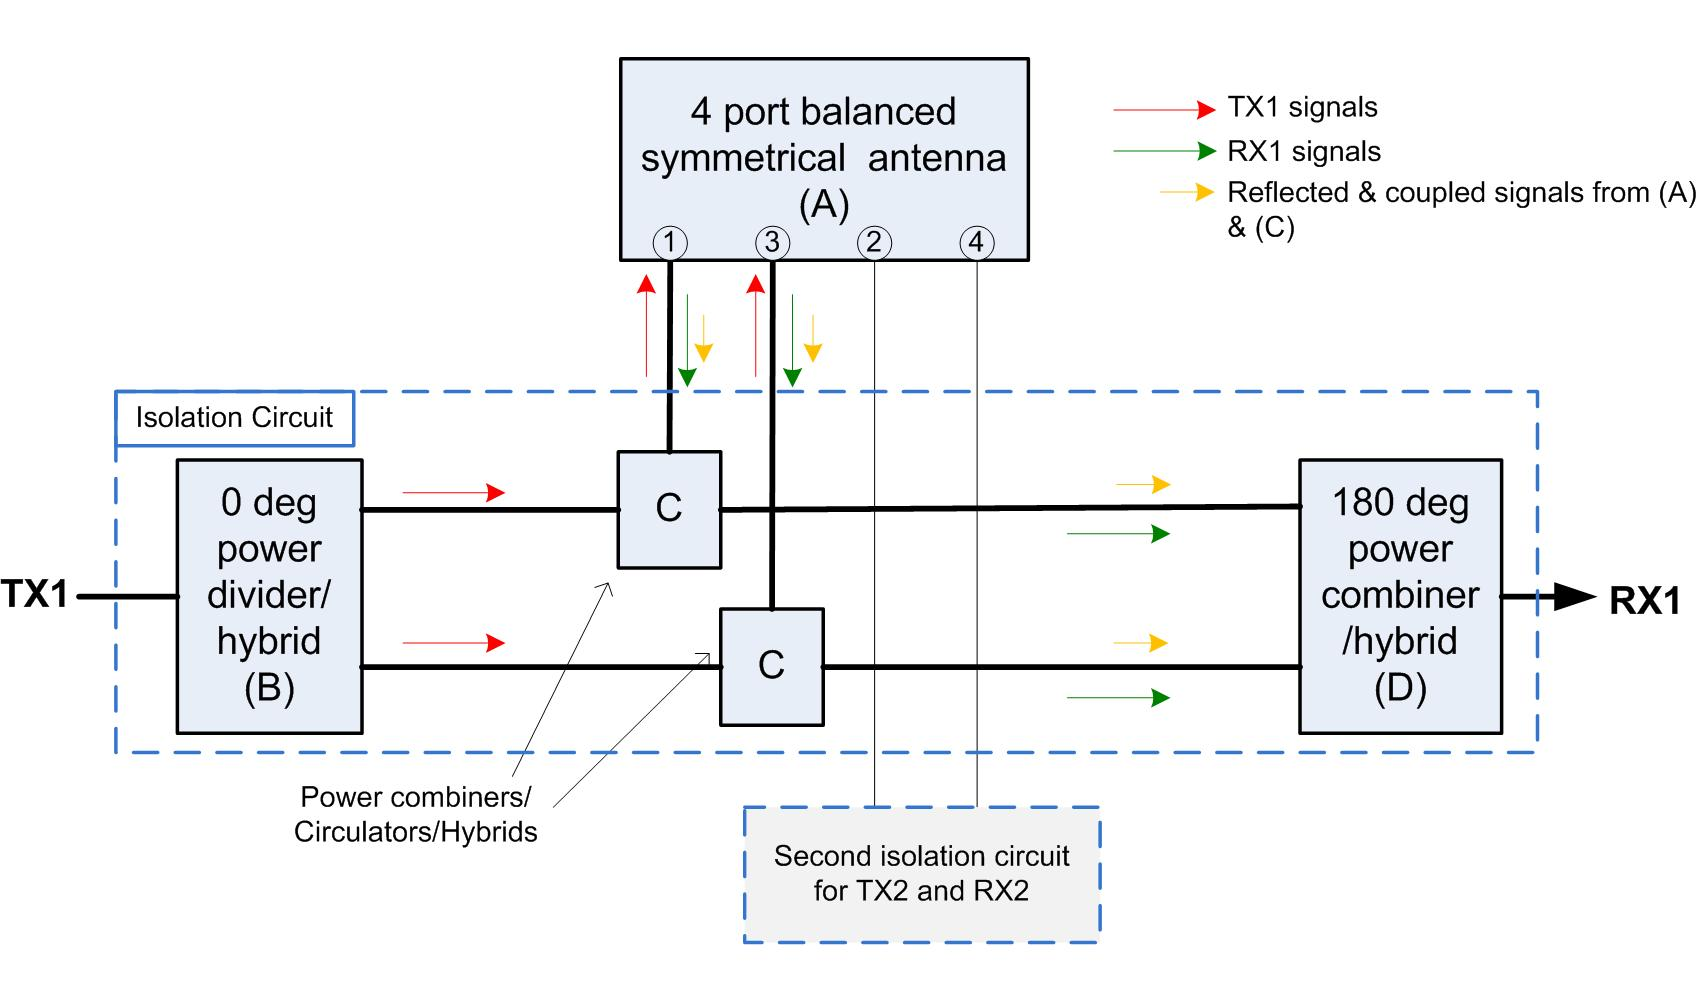
\includegraphics[width=2.5in]{fdmimo2diagram.jpg}
\DeclareGraphicsExtensions.
\caption{Full Duplex 2x2 MIMO Antenna and Isolation Circuit Layout}
\label{fig_mimodiag}
\end{figure} 


\section{Implementation of a Musical Instrument}
\subsection{Frquency Generation}
The source of maintaing high isolation lies in the circulator (noted (C) in Fig.\ref{fig_mimodiag}) which allows a signal to pass only to its neighbor in the clockwise direction. It is desired to replace this component due to the high cost and large volume of manufactured high isolation circulators. For cost effectiveness and ease of fabrication, it was desired to implement a microstrip circuit with few mounted components. The structure considered to provide the required isolation was the circular 180\degree\space hybrid as seen in  Fig.\ref{fig_rrcomb}. Because the segments of the circuit are quarter wavelength multiples, some interesting properties arise depending on the port(s) the signals are applied to. As seen in Fig.\ref{fig_rrcomb}, signals applied at TX1 split evenly to ANT1 and ANT 2 and recombine destructively at RX1, ideally creating perfect isolation at the centre frequency. As well, identical signals applied at ANT1 and ANT2 recombine in phase at RX1 but recombine destructively at TX1, sucessfully splitting the transmit signals to the antennae and recombining the recieved signals at the RX1 port as required. Therefore, by applying the signals at the correct ports, this circuit structure can replace the function of all the isolation circuit components seen in Fig.\ref{fig_mimodiag}. However, due to the wavelength based properties of this structure, high isolation is only achieved at the centre frequency making it extremely narrow band. Work has been done previously on developing wideband 180\degree\space hybrid combiners as demonstrated in multiple papers as well as in the book titled Microwave Ring Circuits and Related Structures \cite{chang_wideband_2012}\cite{taravati_miniaturized_2013}\cite{chiu_compact_2013}\cite{chang_microwave_2004}. Of these designs, the one that seemed the most promising and most simple to fabricate was the structure presented in the paper by Quan Xue and Leung Chiu which regulated the narrow band issue by replacing the 3/4 wavelength section with a 180\degree\space parallel stripline phase shifter, allowing isolation across the band \cite{chiu_compact_2013}. After simulating the structure proposed in \cite{chiu_compact_2013}, there was still significant error in the phase inverter structure, prompting an improvement in this part of the circuit structure.

\begin{figure}[!t]
\centering
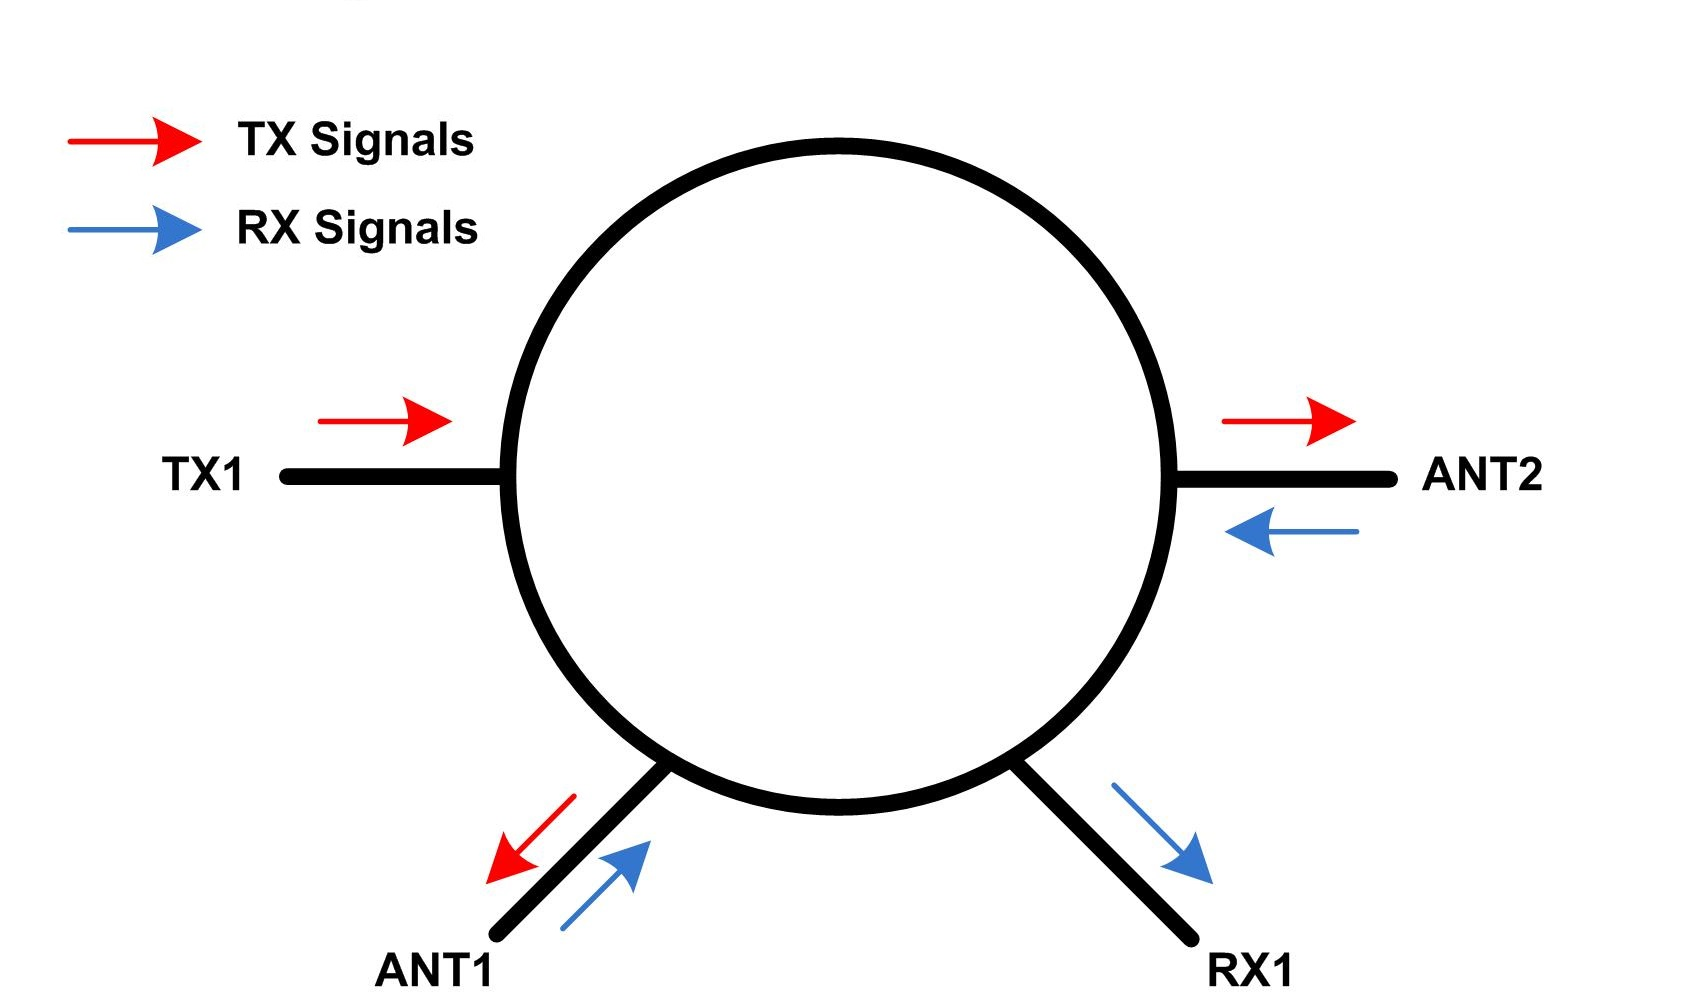
\includegraphics[width=2.5in]{rrcomb.jpg}
\DeclareGraphicsExtensions.
\caption{180\degree\space hybrid combiner properties for 2x2 full duplex MIMO use.}
\label{fig_rrcomb}
\end{figure} 

\subsection{Signal Generation and Processing}
The instrument creates a tone quality for each note by generating the fundamental frequency signal and combining it with the four subsequent harmonics. Since the operations required for signal generation and processing require fast performance, the signal generation and processing logic is designed on the onboard FPGA of the NI MyRio. Fig.\ref{fig_notegen} shows the implementation of signal generation in LabVIEW. Sine wave generator blocks are used to produce a sine wave at a calculated frequency. To produce four subsequent harmonics, the calculated frequency is multiplied by integer factors, two through five, and the resultant frequencies are used as input to separate sine wave generator blocks.  An array of fixed point numbers contain the gain level of each harmonic are converted into a cluster, de-bundled, and then multiplied to the output of their respective sine waves before they are summed together. This allows for variable tone quality by changing the volume of each harmonic. Multiplication is carried out using fixed point arithmetic for increased precision.

Three instances of the signal generation code are used to generate three separate notes. Similar to the harmonic volume each note is multiplied by a fixed point number gain to control the volume of each note. Chords are enabled by a summation of the three separate notes.

Acceleration controlled volume level of the output signal is achieved through scaling the raw acceleration data from the native accelerometer to the NI MyRio, and multiplying the result with the output signal. Similar to signal generation, multiplication is carried out using fixed point numbers for precision. Fig.\ref{fig_accvol} shows the implementation of signal volume control in LabVIEW. A select block controlled by a control is used to switch between the signal at acceleration controlled volume and at maximum volume. Mute functionality is implemented similarly with a select block switching between the generated signal and no signal.


\begin{figure}[!t]
\centering
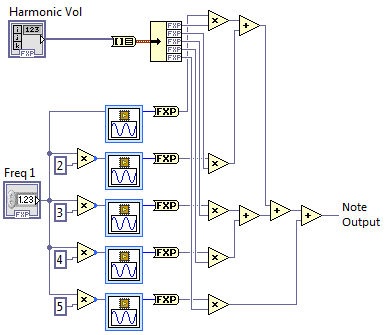
\includegraphics[width=3in]{NoteGeneration.png}
\DeclareGraphicsExtensions.
\caption{LabVIEW code for generating the summation of a sine wave and four of its harmonics.}
\label{fig_notegen}
\end{figure} 

\begin{figure}[!t]
\centering
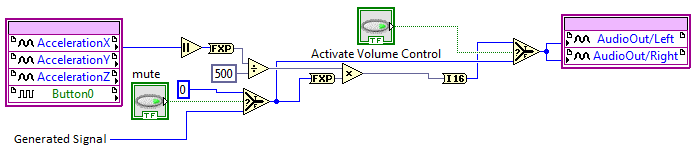
\includegraphics[width=3.5in]{AccelerometerVolume.png}
\DeclareGraphicsExtensions.
\caption{LabVIEW code for changing the gain on the output signal using accelerometer data and controls.}
\label{fig_accvol}
\end{figure} 

\subsubsection{Twisted Line Structure}
One of the simulated inverter structures consisted of cutting a slot in the PCB and fabricating two copper strips which would be individually twisted to connect the opposing top and bottom lines as seen in Fig.\ref{fig_linetwist}. Simulations for this structure showed improvement in both S11 and phase inversion from the original structure. However due to the difficulty in replication of fabrication, this structure was abandoned.

 \begin{figure}[!t]
\centering
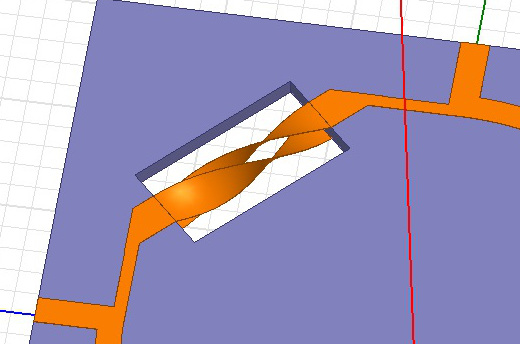
\includegraphics[width=2.5in]{linetwist.jpg}
\DeclareGraphicsExtensions.
\caption{Twisted line phase inverter structure.}
\label{fig_linetwist}
\end{figure} 

\subsubsection{Meandered Line Structure}
Due to the improvements in the previous structure where the line was not cut, it was desired to find a similar method of swapping the top and bottom signals without cutting into the line. Using a variation of the original structure, a straight cut was made all the way through the line and both sections were extended and meandered to end side by side as seen in  Fig.\ref{fig_swerve}. An identical modification was made to the bottom but with the lines meandering in the opposite direction allowing the top and bottom lines to line up. Via holes were added to connect the top and bottom lines. This modification to the structure allowed for the lines to maintain their width as well as allowing for the inclusion of larger via holes. Simulation results revealed this structure to behave similarly to the twisted line structure, but allowed for much more consistency in fabrication.

 \begin{figure}[!t]
\centering
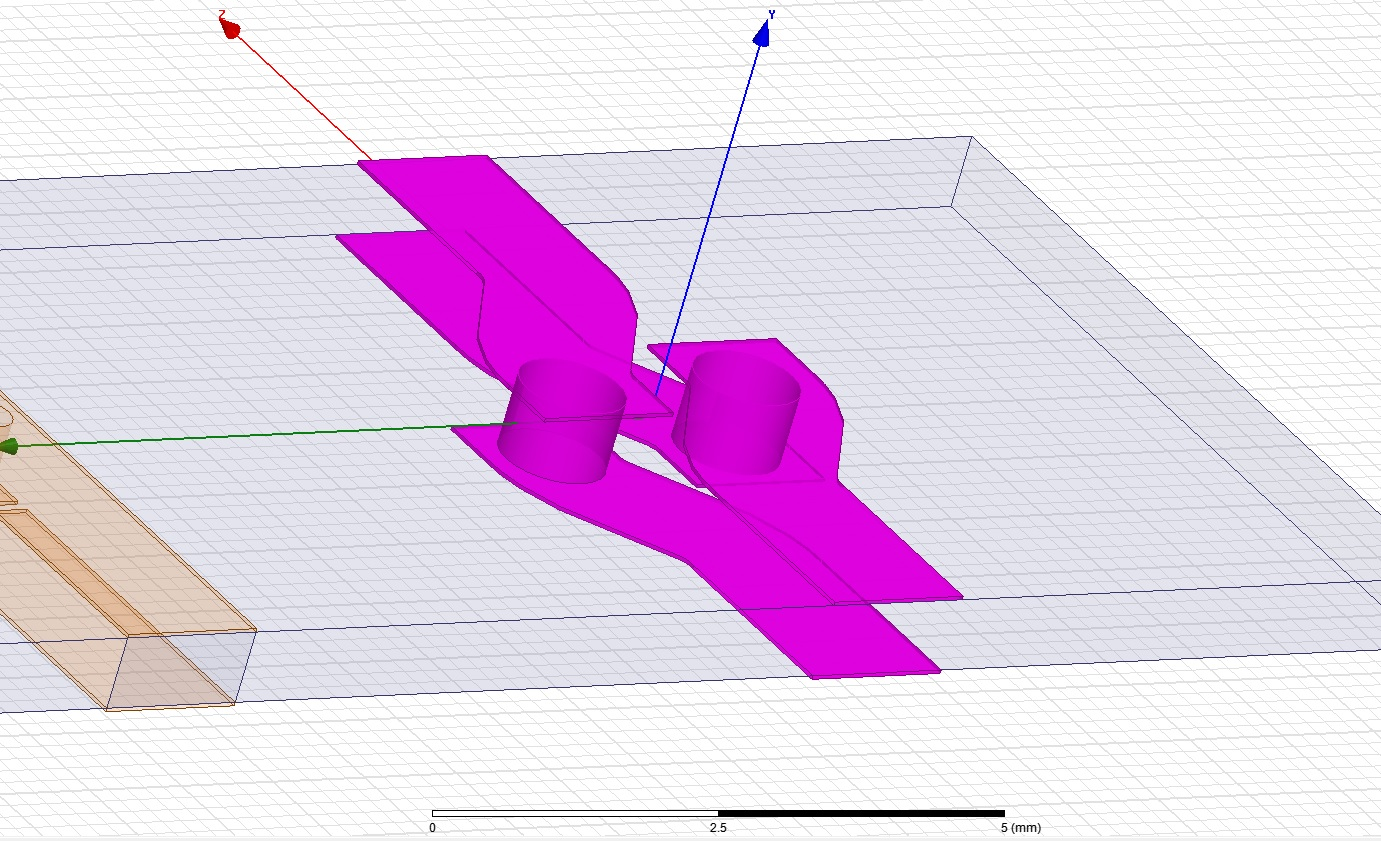
\includegraphics[width=2.5in]{swerve.jpg}
\DeclareGraphicsExtensions.
\caption{Meandered line phase inverter structure.}
\label{fig_swerve}
\end{figure} 

\subsection{Balun Taper}
In order for the balanced parallel stripline structure to make connection with an unbalanced SMA connector, a balanced to unbalanced (balun) taper was needed. Using an approximation of the Klopfenstein taper, this structure was simulated in HFSS until adequate impedance matching results were achieved \cite{rizvi_klopfenstein_2012-1}.

\subsection{Final Assembly and Modifications}
Including both the modified phase inverter structure and the balun taper, the circuit was simulated until optimum results were achieved. Due to the extra path length introduced by the meanedered phase inverter structure and the via hole, the circuit was not exactly symmetric. In order to compensate for this added pathlength, small arcs were added to the other three quarter circle sections. Adjusting the length of these arc sections during simulation yielded the final results seen in Fig.\ref{fig_simresults}. The final circuit structure used can be seen in Fig.\ref{fig_final}.

 \begin{figure}[!t]
\centering
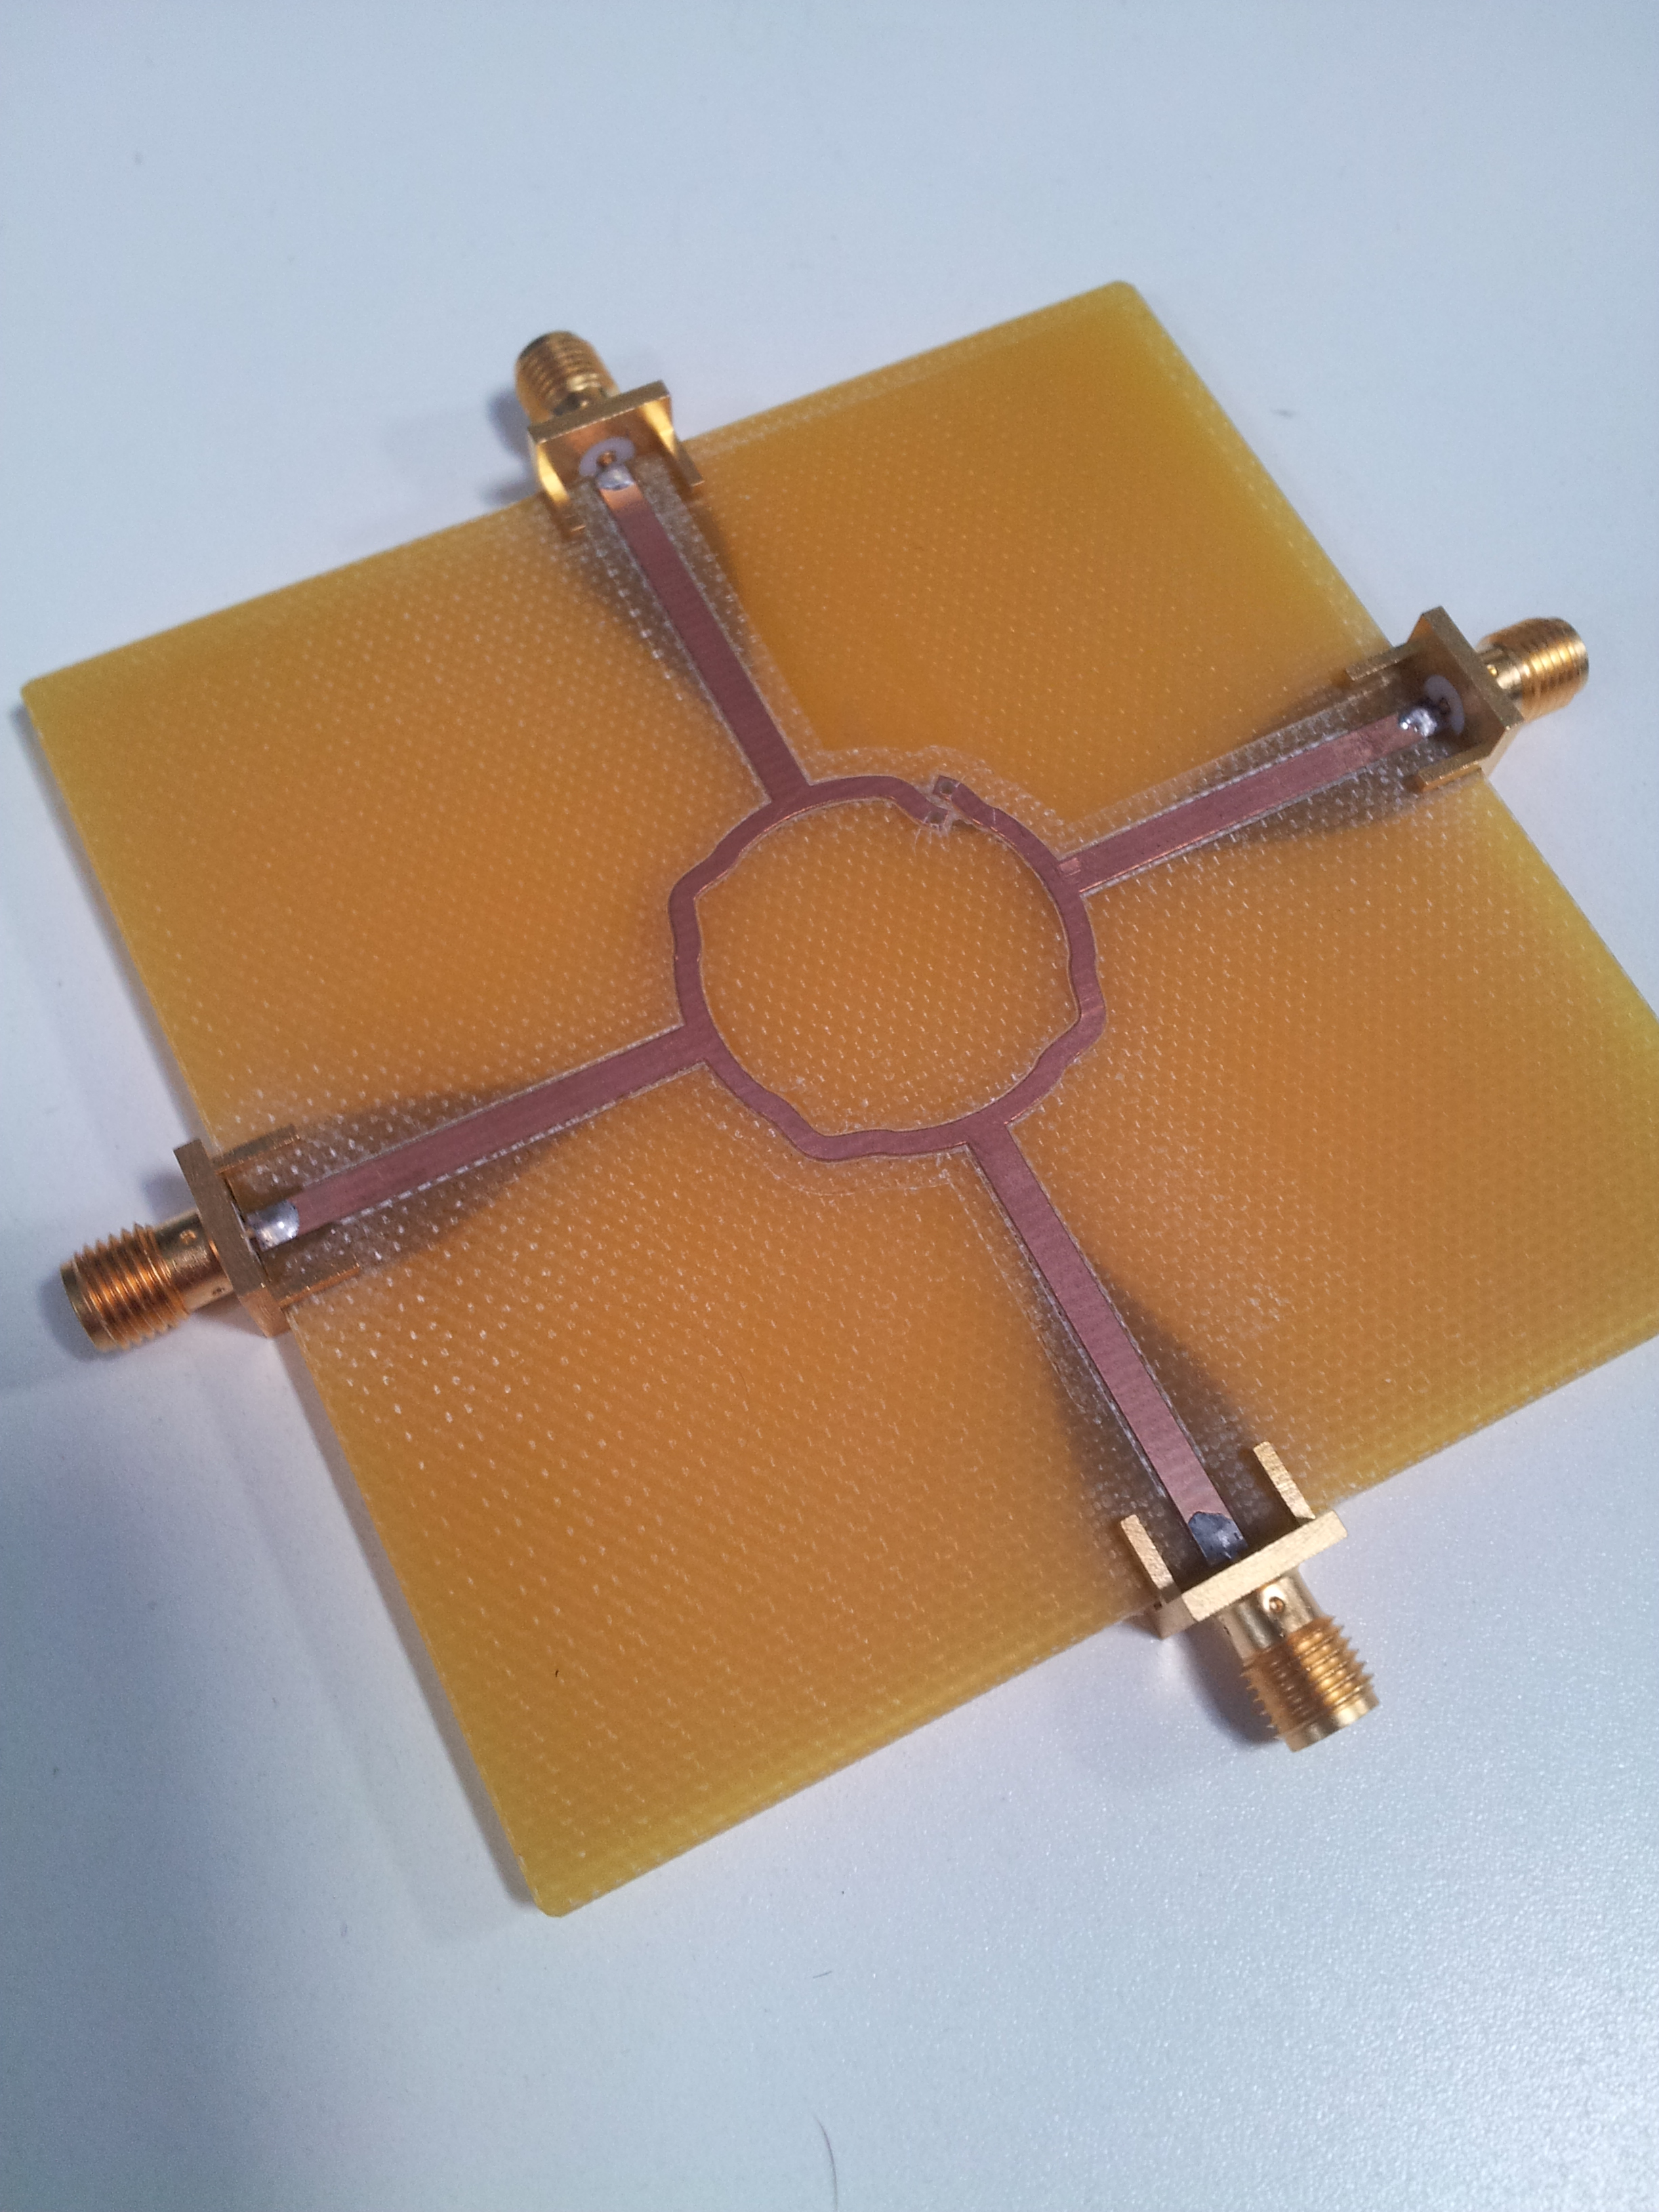
\includegraphics[width=2.5in]{finalfab.jpg}
\DeclareGraphicsExtensions.
\caption{Final fabricated circuit structure with included phase inverter, balun taper and path length correction.}
\label{fig_final}
\end{figure}

\begin{figure}[!t]
\centering
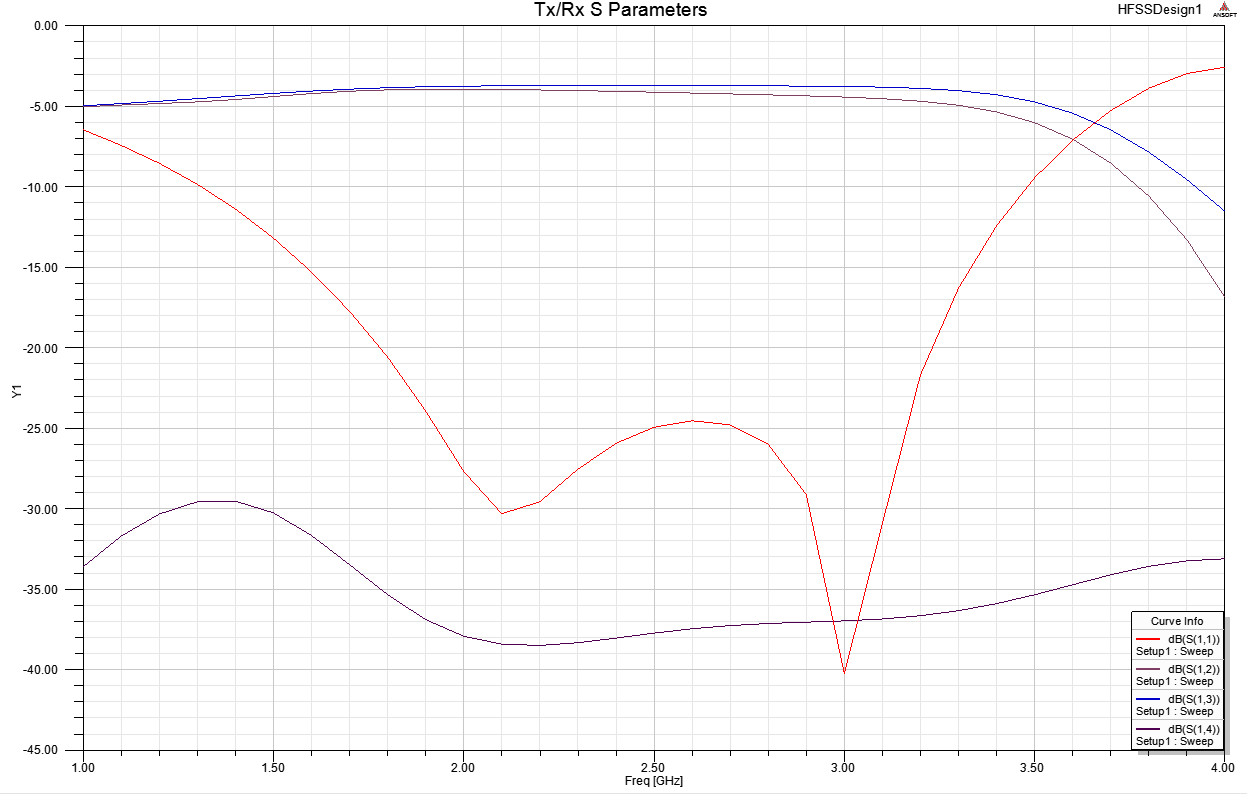
\includegraphics[width=2.5in]{finalsimresults.png}
\DeclareGraphicsExtensions.
\caption{Simulation results from final optimized structure}
\label{fig_simresults}
\end{figure}  

% needed in second column of first page if using \IEEEpubid
%\IEEEpubidadjcol

\section{Results and Discussion}
After optimizing the structure in simulation, a prototype was fabricated as seen in Fig.\ref{fig_final}. The circuit was tested using a VNA and both antenna ports on the circuit connected to 50 ohm terminals. The isolation value S21 was measured from the transmit to the recieve port on the circuit. The results in Fig.\ref{fig_results}  show almost identical behaviour to the final simulation seen in  Fig.\ref{fig_simresults}. It should be noted that these results show approximately 10dB isolation improvent over the structure presented in  \cite{chiu_compact_2013}.

 \begin{figure}[!t]
\centering
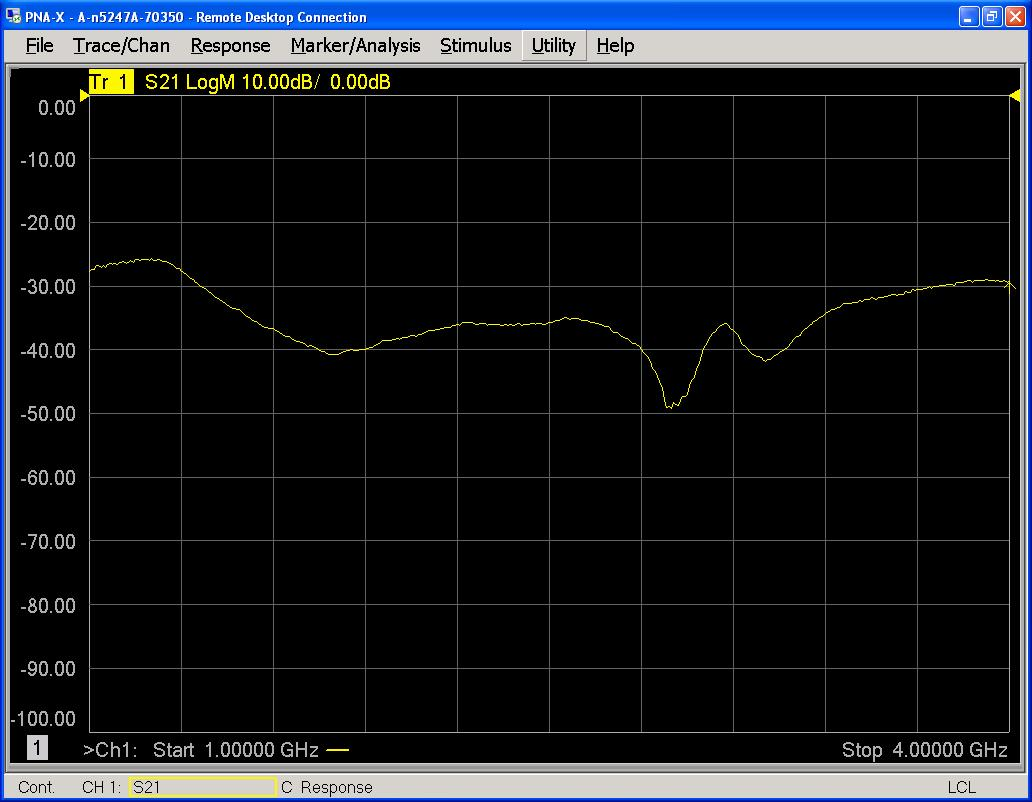
\includegraphics[width=2.5in]{results.jpg}
\DeclareGraphicsExtensions.
\caption{Test results with VNA and terminated antenna ports}
\label{fig_results}
\end{figure} 

% An example of a floating figure using the graphicx package.
% Note that \label must occur AFTER (or within) \caption.
% For figures, \caption should occur after the \includegraphics.
% Note that IEEEtran v1.7 and later has special internal code that
% is designed to preserve the operation of \label within \caption
% even when the captionsoff option is in effect. However, because
% of issues like this, it may be the safest practice to put all your
% \label just after \caption rather than within \caption{}.
%
% Reminder: the "draftcls" or "draftclsnofoot", not "draft", class
% option should be used if it is desired that the figures are to be
% displayed while in draft mode.
%
%\begin{figure}[!t]
%\centering
%\includegraphics[width=2.5in]{myfigure}
% where an .eps filename suffix will be assumed under latex,
% and a .pdf suffix will be assumed for pdflatex; or what has been declared
% via \DeclareGraphicsExtensions.
%\caption{Simulation Results}
%\label{fig_mimodiag}
%\end{figure}

% Note that IEEE typically puts floats only at the top, even when this
% results in a large percentage of a column being occupied by floats.


% An example of a double column floating figure using two subfigures.
% (The subfig.sty package must be loaded for this to work.)
% The subfigure \label commands are set within each subfloat command, the
% \label for the overall figure must come after \caption.
% \hfil must be used as a separator to get equal spacing.
% The subfigure.sty package works much the same way, except \subfigure is
% used instead of \subfloat.
%
%\begin{figure*}[!t]
%\centerline{\subfloat[Case I]\includegraphics[width=2.5in]{subfigcase1}%
%\label{fig_first_case}}
%\hfil
%\subfloat[Case II]{\includegraphics[width=2.5in]{subfigcase2}%
%\label{fig_second_case}}}
%\caption{Simulation results}
%\label{fig_sim}
%\end{figure*}
%
% Note that often IEEE papers with subfigures do not employ subfigure
% captions (using the optional argument to \subfloat), but instead will
% reference/describe all of them (a), (b), etc., within the main caption.


% An example of a floating table. Note that, for IEEE style tables, the
% \caption command should come BEFORE the table. Table text will default to
% \footnotesize as IEEE normally uses this smaller font for tables.
% The \label must come after \caption as always.
%
%\begin{table}[!t]
%% increase table row spacing, adjust to taste
%\renewcommand{\arraystretch}{1.3}
% if using array.sty, it might be a good idea to tweak the value of
% \extrarowheight as needed to properly center the text within the cells
%\caption{An Example of a Table}
%\label{table_example}
%\centering
%% Some packages, such as MDW tools, offer better commands for making tables
%% than the plain LaTeX2e tabular which is used here.
%\begin{tabular}{|c||c|}
%\hline
%One & Two\\
%\hline
%Three & Four\\
%\hline
%\end{tabular}
%\end{table}


% Note that IEEE does not put floats in the very first column - or typically
% anywhere on the first page for that matter. Also, in-text middle ("here")
% positioning is not used. Most IEEE journals use top floats exclusively.
% Note that, LaTeX2e, unlike IEEE journals, places footnotes above bottom
% floats. This can be corrected via the \fnbelowfloat command of the
% stfloats package.



\section{Conclusion and Future Improvements}
A modified 180\degree\space hybrid combiner for use in broadband 2x2 MIMO applications was presented and developed as an isolation circuit to be used with a symmetrical 4 port antenna. The structure proposed in (reference) was improved upon and applied to full duplex applications. While this circuit structure is effective and extremely inexpensive to manufacture, with a TX/RX isolation of only -38dB it still needs  improvement before it can be sucessfully applied to long range communications. With more time to develop and simulate this circuit structure, this isolation level could be improved and tested with the 4 port antenna.





% if have a single appendix:
%\appendix[Proof of the Zonklar Equations]
% or
%\appendix  % for no appendix heading
% do not use \section anymore after \appendix, only \section*
% is possibly needed

% use appendices with more than one appendix
% then use \section to start each appendix
% you must declare a \section before using any
% \subsection or using \label (\appendices by itself
% starts a section numbered zero.)
%





% use section* for acknowledgement
\section*{Acknowledgment}


Thank you to my supervisors Thanh Ngon Tran and Robert Morawski as well as fellow undergraduate student Harry Lee and Prof. Tho Le-Ngoc for all the guidance and support.

% trigger a \newpage just before the given reference
% number - used to balance the columns on the last page
% adjust value as needed - may need to be readjusted if
% the document is modified later
%\IEEEtriggeratref{8}
% The "triggered" command can be changed if desired:
%\IEEEtriggercmd{\enlargethispage{-5in}}

% references section

% can use a bibliography generated by BibTeX as a .bbl file
% BibTeX documentation can be easily obtained at:
% http://www.ctan.org/tex-archive/biblio/bibtex/contrib/doc/
% The IEEEtran BibTeX style support page is at:
% http://www.michaelshell.org/tex/ieeetran/bibtex/
\bibliographystyle{ieeetran}
% argument is your BibTeX string definitions and bibliography database(s)
\bibliography{references}
%
% <OR> manually copy in the resultant .bbl file
% set second argument of \begin to the number of references
% (used to reserve space for the reference number labels box)


% biography section


\end{document}



